
\chapter{ಸರ್ವೇ ಸಮಸ್ಯೆಗಳ ಸರಮಾಲೆ ಕರ್ನಲ್​ ಜಾರ್ಜ್ ಎವರೆಸ್ಟ್​ರ ಕೊರಳಿಗೆ}

\vskip -9pt

ಸರ್ವೇ ಕಾರ್ಯವೆಂದರೆ ಅದು ಸಮಸ್ಯೆಗಳ ಸರಮಾಲೆ. ದಟ್ಟ ಕಾಡಿನಲ್ಲಿ, ಸುರಿಯುವ ಮಳೆಯಲ್ಲಿ, ಸುಡುವ ಬಿಸಿಲಿನಲ್ಲಿ, ವಯಕ್ತಿಕ ಸುರಕ್ಷತೆಯನ್ನು ಕಡೆಗಣಿಸಿ ಅಪಾಯದ ಅಂಚಿನಲ್ಲಿ ಕಾರ್ಯ ನಿರ್ವಹಿಸಬೇಕು. ಲ್ಯಾಂಬ್​ಟನ್​ರವರು ಎದುರಿಸಬೇಕಾದ ಸಮಸ್ಯೆಗಳು ಬರಿ ಕ್ಷೇತ್ರಕಾರ್ಯದ ಕಷ್ಟನಷ್ಟಗಳು ಮಾತ್ರ ಆಗಿರಲಿಲ್ಲ. ಅವರ ಸರ್ವೇಯ ಉಪಯುಕ್ತತೆಯನ್ನು ಆಡಳಿತ ವರ್ಗಕ್ಕೆ ಪದೇ ಪದೇ ವಿವರಣೆ ನೀಡುತ್ತಾ, ಅದರ ಅಗತ್ಯವನ್ನು, ಮೇಲಿಂದ ಮೇಲೆ ರುಜುವಾತು ಪಡಿಸುತ್ತಿರಬೇಕಾಗಿತ್ತು. ಬಂಗಾಳದ ಸರ್ವೇಯರ್​ ಜನರಲ್​ ಆಗಿದ್ದ ಮೇಜರ್​ ರನೆಲ್​ರವರೇ ಮುಂದೆ ಬಂದು, ಲ್ಯಾಂಬ್​ಟನ್​ರವರ ಗಣಿತೀಯ ಸರ್ವೇಗೆ ತಮ್ಮ ವಿರೋಧ ಅಭಿಪ್ರಾಯವನ್ನು ನೀಡಿದರು. ಮ್ಯಾಪಿಂಗ್​ ಕಾರ್ಯದಲ್ಲಿ ರನ್ನೆಲ್​ರವರದ್ದು ಬಹು ದೊಡ್ಡ ಹೆಸರು. ಖಗೋಳ ವೀಕ್ಷಣೆಯನ್ನು ಆಧರಿಸಿದ ರೂಟ್​ ಸರ್ವೆಯು ಸಹ, ಸಮಾನ ನಿಖರತೆಯನ್ನು ನೀಡಬಲ್ಲದು ಹಾಗೂ ಆ ಕ್ರಮವೇ ಹೆಚ್ಚು ಮಿತವ್ಯಯಕಾರಿ ಎಂಬುದು ರನೆಲ್​ರವರ ವಾದ. ಜೊತೆಗೆ, ಮದರಾಸಿನ ಆರ್ಥಿಕ ಸಮಿತಿಯು ಸಹ ಲ್ಯಾಂಬ್​ಟನ್​ರವರ ಸಾಧನ ಸಂಪನ್ಮೂಲಗಳನ್ನು ಕುಂಠಿತಗೊಳಿಸಿತು. ಯುರೋಪಿನ ವಿಜ್ಞಾನ ಸಂಸ್ಥೆಗಳು ಆರಂಭದಲ್ಲಿ ಅಗತ್ಯವಿದ್ದ ಬೆಂಬಲ ಪ್ರೋತ್ಸಾಹ ನೀಡಲಿಲ್ಲ. ಲ್ಯಾಂಬ್​ಟನ್​ರವರಿಗೆ ಬ್ರಿಟೀಷ್​ ಸರ್ಕಾರದಿಂದಾಗಲೀ, ರಾಯಲ್​ ಸೊಸೈಟಿಯಿಂದಾಗಲೀ ಒಂದೇ ಒಂದು ಸಹಾನುಭೂತಿಯ ನುಡಿ ಬರಲಿಲ್ಲ. ಉತ್ತೇಜಕ ಸಲಹೆ ಸೂಚನೆ ಮಾತು ಸಿಗಲಿಲ್ಲ. ಇದು ಯಾವುದನ್ನೂ ಮನಸ್ಸಿಗೆ ತಂದುಕೊಳ್ಳದೇ ಅವರು ತಮ್ಮ ಗ್ರೇಟ್​ ಆರ್ಕ್‌ನ ಟ್ರೈಯಾಂಗ್ಯುಲೇಷನ್​ ಕಾರ್ಯದಲ್ಲಿ ಮೌನವಾಗಿ ಮುಳುಗಿದ್ದರು.

ಅಂತಿಮವಾಗಿ, \enginline{1818}ರಲ್ಲಿ ಲ್ಯಾಂಬ್​ಟನ್​ರವರು ರಾಯಲ್​ ಸೊಸೈಟಿಯ ಫೆಲೋ ಆಗಿ ಆಯ್ಕೆ ಆದರು. ಇವರ ಸರ್ವೇಯ ಮಹತ್ವವನ್ನು ಅರಿತು, ಸರಕಾರವು ಇವರ ಸರ್ವೆಯನ್ನು “ಗ್ರೇಟ್​ ಟ್ರಿಗನಮಿಟ್ರಿಕಲ್​ ಸರ್ವೆ ಆಫ್​ ಇಂಡಿಯ” ಎಂದು ಕರೆಯಿತು. ಈ ಯೋಜನೆಯ ಬಲವರ್ಧನೆಯ ಭಾಗವಾಗಿ, ಅದೇ ವರ್ಷ, ಗ್ರೇಟ್​ ಟ್ರಿಗನಮಿಟ್ರಿಕಲ್​ ಸರ್ವೆಯ ಉಸ್ತುವಾರಿಯನ್ನು ಮದ್ರಾಸ್​ ಸರಕಾರದಿಂದ ಕೊಲ್ಕತ್ತಾ ಕೇಂದ್ರಕ್ಕೆ ವರ್ಗಾಯಿಸಲಾಯಿತು. ಇದಲ್ಲದೆ, ಕ್ಯಾಪ್ಟನ್​ ಜಾರ್ಜ್ ಎವರೆಸ್ಟ್​ರವರನ್ನು \enginline{1818} ರಲ್ಲಿ ಲ್ಯಾಂಬ್​ಟನ್​ರವರಿಗೆ ಸಹಾಯಕರಾಗಿ, ಗ್ರೇಟ್​ ಟ್ರಿಗನಮಿಟ್ರಿಕಲ್​ ಸರ್ವೆ ಆಫ್​ ಇಂಡಿಯಾದ ಸಹಾಯಕ ಅಧೀಕ್ಷಕರಾಗಿ ಹೊಸದಾಗಿ ನೇಮಿಸಲಾಯಿತು. ಜೊತೆಗೆ ಡಾ. ವಾಯ್ಸೆರವರನ್ನು ಸರ್ವೇ ತಂಡದ ವೈದ್ಯಕೀಯ ಸಹಾಯಕ ಹಾಗೂ ಭೂವಿಜ್ಞಾನಿಯನ್ನಾಗಿಯೂ ಸಹ ನೇಮಿಸಲಾಯಿತು.

\enginline{1818}ರ ಅಂತಿಮ ಭಾಗದಲ್ಲಿ ತರುಣ ಎವರೆಸ್ಟ್​ರವರು, ಲ್ಯಾಂಬ್​ಟನ್​ರವರನ್ನು\break ಹೈದರಾಬಾದಿನಲ್ಲಿ ಟ್ರಿಗನಮಿಟ್ರಿಕಲ್​ ಸರ್ವೇ ಕಾರ್ಯದಲ್ಲಿ ಜೊತೆಗೂಡಿದರು. ಎವರೆಸ್ಟ್​\break ರವರು ತಮ್ಮ ಮೇಲಧಿಕಾರಿ ಲ್ಯಾಂಬ್​ಟನ್​ರವರನ್ನು ಅದೇ ಮೊದಲ ಬಾರಿಗೆ ನೋಡಿದ್ದು. ಆಗ ಲ್ಯಾಂಬ್​ಟನ್​ರವರಿಗೆ \enginline{66}ರ ಹರಯ. ಆರು ಅಡಿ ಎತ್ತರವಿದ್ದ ಗುರು ಲ್ಯಾಂಬ್​ಟನ್​\break ರವರು, ಶಿಷ್ಯ ಎವರೆಸ್ಟ್​ರವರಿಗೆ, ಸುಂದರವಾಗಿ, ಆರೋಗ್ಯವಾಗಿ, ದೃಢಕಾಯರಾಗಿಯೇ ಕಂಡರು. ಆದರೂ ಸಹ ಸರ್ವೇ ಕ್ಷೇತ್ರ ಕಾರ್ಯದ ನಿರಂತರ ಕಠಿಣ ದುಡಿಮೆಯಿಂದ ಅವರು ದಣಿದಿದ್ದರು. ಎಷ್ಟೇ ಧಣಿದಿದ್ದರೂ ಸಹ ಮ್ಯಾಪಿಂಗ್​ ಮಹಾ ಕಾರ್ಯದಿಂದ ವಿಶ್ರಮಿಸಿಕೊಳ್ಳುವ ಯೋಚನೆಯನ್ನು ಲ್ಯಾಂಬ್​ಟನ್​ರವರು ಮಾಡಲೇ ಇಲ್ಲ. ಗ್ರೇಟ್​ ಆರ್ಕ್‌ನ ಟ್ರೈಯಾಂಗ್ಯುಲೇಷನ್​ ಕಾರ್ಯದ ತಮ್ಮ ನಿತಂತರ ತಪೋ ಕಾರ್ಯದಲ್ಲಿ ಮೌನವಾಗಿ ಮುಳುಗಿದ್ದರು.

ಲ್ಯಾಂಬ್​ಟನ್​ರವರಿಗೆ ಮುಖ್ಯ ಸಹಾಯಕರಾಗಿ ನೇಮಕವಾದ ಎವರೆಸ್ಟ್​ರವರು ಲಂಡನ್ನಿನ ಸಮಿಪದ ಗ್ರೀನಿಚ್​ನವರು. ಗ್ರೀನಿಚ್​ ಪಟ್ಟಣವು ರಾಯಲ್​ ಖಗೋಳ ವೀಕ್ಷಣಾಲಯ ಇರುವ, ಪ್ರಧಾನ ರೇಖಾಂಶ ರೇಖೆಯು ಹಾದು ಹೋಗುವ ಜಿಯೋಗ್ರಫಿಯ ತವರೂರು. ಈ ಊರು ಗ್ರೇಟ್​ ಬ್ರಿಟನ್​ ದೇಶದ ಥೇಮ್ಸ ನದಿಯ ದಂಡೆಯ ಮೇಲಿದೆ. \enginline{2}ನೇ ಚಾರ್ಲ್ಸ್ ದೊರೆಯು \enginline{1675}ರಲ್ಲಿ ಸ್ಥಾಪಿಸಿದ ಮೂಲ ರಾಯಲ್​ ಖಗೋಳ ವೀಕ್ಷಣಾಲಯ ಇದ್ದ ಸ್ಥಳ ಇದು. ಈ ಗ್ರೀನಿಚ್​ ಪಟ್ಟಣವನ್ನು ಪ್ರಧಾನ ರೇಖಾಂಶ ರೇಖೆ ಹಾದು ಹೋಗುವ ಸ್ಥಳವೆಂದು \enginline{1884} ರಿಂದ ಅಂತರಾಷ್ಟ್ರೀಯವಾಗಿ ಒಪ್ಪಿ ಸ್ವೀಕರಿಸಲಾಗಿದೆ. ಈ ಪಟ್ಟಣದ ಮೇಲೆ ಹಾದು ಹೋಗುವ ರೇಖಾಂಶವನ್ನು ಗ್ರೀನಿಚ್​ ರೇಖಾಂಶವೆಂದು ಕರೆಯಲಾಗಿದೆ. ಇದು ಸೊನ್ನೆ ಡಿಗ್ರಿ ರೇಖಾಂಶವಾಗಿದ್ದು, ರೇಖಾಂಶಗಳ ಎಣಿಕೆ ಇಲ್ಲಿಂದಲೇ ಆರಂಭವಾಗುತ್ತದೆ. ರಾಯಲ್​\break ವೀಕ್ಷಣಾಲಯವನ್ನು \enginline{1948}ರಲ್ಲಿ ಹರ್ಟ್ಸ್‌ಮನ್ಸ್ಯೂಗೆ ವರ್ಗಾಯಿಸಲಾಯಿತಾದರೂ, ಮೊದಲಿನಂತೆ ರೇಖಾಂಶ ಎಣಿಕೆಯ ಕ್ರಮ ಮಾತ್ರ ಈಗಲೂ ಇಲ್ಲಿಂದಲೇ ಪ್ರಾರಂಭವಾಗುತ್ತದೆ.

ಎವರೆಸ್ಟ್​ರವರು ಅಲ್ಲಿನ ವೂಲ್​ವಿಚ್​ ರಾಯಲ್​ ಮಿಲಿಟರಿ ಅಕಾಡೆಮಿಯಲ್ಲಿ ಗಣಿತ, ಮೆಕಾನಿಕ್ಸ್​ ಮತ್ತು ಮಿಲಿಟರಿಗೆ ಅಗತ್ಯವಾದ ಸರ್ವೇ ಈ ವಿಚಾರಗಳನ್ನು ಕಲಿತವರು. ಗ್ರೇಟ್​ ಟ್ರಿಗನಮಿಟ್ರಿಕಲ್​ ಸರ್ವೇಗೆ ಇವರ ನೇಮಕವು ಇವರಿಗೊಂದು ಮಹಾ ಸದವಕಾಶವೇ ಅಗಿತ್ತು. ಇಂಗ್ಲಿಷ್​ ಲೆಫ್ಟಿನೆಂಟ್​ ಕರ್ನಲ್​ ಜಾರ್ಜ್ ಎವರೆಸ್ಟ್​ರವರು, ತಮ್ಮ ಸರ್ವೇ ಕಾರ್ಯದ ಈ ನೂತನ ಜವಾಬ್ದಾರಿಯಲ್ಲಿ ಗುರುತು ಮೂಡಿಸುವ ಏರು ಹುರುಪಿನಲ್ಲಿದ್ದರು. ಆಗ ಅವರು \enginline{28} ವರ್ಷದ ಬಿಸಿ ರಕ್ತದ ತರುಣ.

ಉತ್ತರ–ದಕ್ಷಿಣ ಮತ್ತು ಪೂರ್ವ–ಪಶ್ಚಿಮ ದಿಕ್ಕಿನ ಸರಣಿ ತ್ರಿಭುಜಗಳ ಪಟ್ಟಿಗಿಂತ ಇಡೀ ಪರ್ಯಾಯ ದ್ವೀಪವನ್ನು ಆವರಿಸಿರುವ ತ್ರಿಭುಜಗಳ ಜಾಲವು ಮ್ಯಾಪ್​ ಕಾರ್ಯಕ್ಕೆ ಅಗತ್ಯ ಆಧಾರ ಆಗಿರಬೇಕು ಎಂದು ಕಂಪನಿ ಸರಕಾರವು ಸೂಚಿಸಿತ್ತು. ಈ ಕಾರಣಕ್ಕೆ\break ಲ್ಯಾಂಬ್​ಟನ್​ರವರು, ತಮ್ಮ ಮುಖ್ಯ ಹೊಸ ಸಹಾಯಕ ಎವರೆಸ್ಟ್​ರವರನ್ನು ಜೂನ್​ \enginline{1819} ರಲ್ಲಿ ಹೈದರಾಬಾದಿನ ಕೃಷ್ಣಾ ಗೋದಾವರಿ ನದಿಗಳ ನಡುವಿನ ಪ್ರದೇಶದಲ್ಲಿ, ಸೆಕೆಂಡರೀ ಟ್ರಾಂಗ್ಯುಲೇಶನ್​ ಕಾರ್ಯಕ್ಕೆ ನಿಯೋಜಿಸಿದರು. ಮಧ್ಯ ಭಾರತದ ಆ ಪ್ರದೇಶವು ಇನ್ನೂ ಅಸ್ಥಿರ ರಾಜ್ಯವಾಗಿತ್ತು. ಕೆಲವು ಜಿಲ್ಲೆಗಳು ನಿಜಾಮ್ ಸರಕಾರದ ವಿರುದ್ಧ ಬಂಡಾಯ ಎದ್ದಿದ್ದವು. ಇಂತಹ ಪ್ರದೇಶದಲ್ಲಿ ತಮ್ಮ ದುರಂತಮಯ ಮೊದಲ ಸರ್ವೇ ಕಾರ್ಯವನ್ನು ಎವರೆಸ್ಟ್​ರವರು ಪ್ರಾರಂಭಿಸಿದರು. ಈ ರಾಜಕೀಯ ಅಶಾಂತ ಸ್ಥಿತಿಯನ್ನು ದಾಟಿ ತಮ್ಮ ಸೆಕೆಂಡರೀ ಟ್ರೈಯಾಂಗ್ಯುಲೇಶನ್​ ಕಾರ್ಯದಲ್ಲಿ ಮುಂದುವರೆದರು.

\begin{figure}[!htbp]
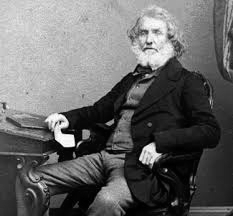
\includegraphics{"images/image012.jpg"}
\caption{ಲೆಫ್ಟಿನೆಂಟ್​ ಕರ್ನಲ್​ ಸರ್​ ಜಾರ್ಜ್ ಎವರೆಸ್ಟ್​}\label{chap8-fig1}
\end{figure}

\newpage

\enginline{28} ವರ್ಷದ ಕರ್ನಲ್​ ಎವರೆಸ್ಟ್​ರವರಿಗೆ ಆರಂಭದಲ್ಲೇ ತಂಡದ ವಿರೋಧವು ಎದು\break ರಾಯಿತು. ಸೇರಿದ ಒಂದು ತಿಂಗಳಲ್ಲೇ ತಮ್ಮ ತಂಡದ ಬಂಡಾಯದ ಬಿಸಿಯನ್ನು ಎದುರಿಸಬೇಕಾಯಿತು. ಅವರ ಬೆಂಗಾವಲು ತಂಡಕ್ಕೆ ಮಳೆಗಾಲದ ಕಾಡಿನ ಅಪಾಯ ಮೊದಲೇ ತಿಳಿದಿತ್ತು. ಆದ್ದರಿಂದ ಬೆಂಗಾವಲು ತಂಡದವರು, ಹೈದರಬಾದ್​ ಕ್ಯಾಂಪ್​ ಬಿಟ್ಟು, ದಟ್ಟ ಕಾಡಿನ ಸರ್ವೇ ಕ್ಯಾಂಪಿಗೆ ಹೋಗಲು ಹಿಂದೇಟು ಹಾಕುತ್ತಾ, ಸಣ್ಣ ನೆಪಕ್ಕಾಗಿ ಕಾಯುತ್ತಿದ್ದರು. ಇದೇ ಸಮಯದಲ್ಲಿ ಗೈರು ಹಾಜರಾದ ಒಬ್ಬನಿಗೆ ಎವರೆಸ್ಟ್​ರವರು ಚಾಟಿ ಏಟಿನ ದೈಹಿಕ ಶಿಕ್ಷೆಯನ್ನು ಆದೇಶಿಸಿದರು. ಬೆಂಗಾವಲು ಪಡೆಗೆ ಇಷ್ಟೇ ಸಾಕಾಯಿತು. ಇಡೀ ಬೆಂಗಾವಲು ಪಡೆ, ಸುಮಾರು \enginline{40} ಜನರ ಗುಂಪು, ತಮ್ಮ ಆಯುಧಗಳನ್ನು ಎತ್ತಿಕೊಂಡು, ಸಾಮೂಹಿಕವಾಗಿ ಕ್ಯಾಂಪ್​ ತೊರೆಯುವುದಾಗಿ ಘೋಷಿಸಿತು.

ಆಗ ಹೈದರಾಬಾದ್​ ಒಂದು ಸಂಸ್ಥಾನೀಯ ರಾಜ್ಯವಾಗಿತ್ತು. ಈ ಸಂಸ್ಥಾನೀಯ ರಾಜ್ಯದಲ್ಲಿ, ಗ್ರೇಟ್​ ಟ್ರಿಗನಮಿಟ್ರಿಕಲ್​ ಸರ್ವೇ ಕಾರ್ಯಾಚರಣೆಗೆ ವಿಶೇಷ ಅನುಮತಿಯನ್ನು ಪಡೆಯಲಾಗಿತ್ತು. ಹೈದರಾಬಾದಿನ ರಾಜ, ನಿಜಾಮ ಸಿಕಂದರ್​ ಝಾ ರವರು ಈ ಬ್ರಿಟೀಷ್​ ಸರ್ವೇಯ ಸಹಾಯಕ್ಕೆ ಮತ್ತು ರಕ್ಷಣೆಗೆಂದು ಒಂದು ಬೆಂಗಾವಲು ಪಡೆಯನ್ನು ನೀಡಿದ್ದರು. ಆ ತುಕಡಿಯೇ ಈಗ ಬಂಡಾಯವೆದ್ದ ತಂಡ. ಬ್ರಿಟೀಷ್​ ಸರ್ವೇ ಅಧಿಕಾರಿಗಳ ರಕ್ಷಣೆಗೆ, ಬ್ರಿಟೀಷ್​ರವರದ್ದೇ ಆದ \enginline{12} ಜನರ, ವಿಶೇಷ ಬೆಂಗಾವಲು ಪಡೆಯೂ ಇತ್ತು. ಈ ವಿಶೇಷ ಪಡೆಯನ್ನು ಬಂಡಾಯವೆದ್ದ ತುಕಡಿಯ ಸದ್ದನ್ನು ಅಡಗಿಸಲು ಬಳಸಲಾಯಿತು. ತುಪಾಕಿಗಳಿಗೆ ಮದ್ದು ಗುಂಡುಗಳನ್ನು ತುಂಬಿ, ಬಂಡಾಯ ಗುಂಪಿನತ್ತ ಗುರಿ ಇರಿಸಲಾಯಿತು. ಎಲ್ಲರೂ ತಕ್ಷಣ ಶರಣಾಗದಿದ್ದರೆ, ಇಡೀ ಗುಂಪಿನ ಮೇಲೆ ತುಪಾಕಿ ಗುಂಡಿನ ಸುರಿಮಳೆಗೈಯುವುದಾಗಿ ಬೆದರಿಸಲಾಯಿತು. ಬ್ರಿಟೀಷ್​ ತಂತ್ರ ಫಲಿಸಿತು. ಅಧಿಕಾರ ಮತ್ತು ತುಪಾಕಿಯ ಮುಂದೆ, ಬರಿಗೈಯ ಬಂಡಾಯ ಸೋತಿತು. ದಂಗೆ ಎದ್ದವರು ತಣ್ಣಗಾಗಿ ಶರಣಾದರು. ಅವರಲ್ಲಿ ಮೂವರಿಗೆ ಸಾರ್ವಜನಿಕವಾಗಿ ಚಡಿ ಏಟು ನೀಡಿ, ಕೆಲಸದಿಂದ ವಜಾಗೊಳಿಸಲಾಯಿತು. ಇದು ಹೈದರಾಬಾದಿನ ನಿಜಾಮರ ನಾಡಿನಲ್ಲಿ ಆರಂಭದಲ್ಲೇ ಎವರೆಸ್ಟ್​ರವರಿಗೆ ಎದುರಾದ ಕಹಿ ಅನುಭವ.

ಟ್ರಿಗನಮಿಟ್ರಿಕಲ್​ ಸರ್ವೇಯಲ್ಲಿ ಮುಖ್ಯವಾದ ಒಂದು ಕಾರ್ಯವೆಂದರೆ, ಈಗಿರುವ ತಾಣದಿಂದ, ಅದರ ಮುಂದಿನ ಕನಿಷ್ಠ \enginline{20–30} ಮೈಲು ದೂರದಲ್ಲಿ ಇರುವ ತೆಳುವಾದ ಸರ್ವೇ ಸ್ತಂಭವನ್ನು ವೀಕ್ಷಣೆ ಮಾಡುವುದು. ಈ ವೀಕ್ಷಣಾ ಕಾರ್ಯವನ್ನು, ಮಳೆಗಾಲ ಮುಗಿದ ತಕ್ಷಣವೇ ನಡೆಸಬೇಕು. ವಾತಾವರಣವು ಆ ಸಮಯದಲ್ಲಿ, ಹೊಗೆ ದೂಳು ರಹಿತವಾಗಿ, ಆಕಾಶವು ಶುಭ್ರವಾಗಿರುತ್ತದೆ. ಮಳೆಗಾಲದ ಸಮಯವು ಸರ್ವೇ ತಂಡಕ್ಕೆ ಬಾರೀ ಅನಾನುಕೂಲ. ಆದರೂ ಸ್ಟೇಷನ್​ ವೀಕ್ಷಣೆಗೆ ಮಾತ್ರ ಅದೇ ಸಂಪೂರ್ಣ ಸೂಕ್ತವಾದ ಕಾಲ. ಸರ್ವೇ ಕಾರ್ಯದಲ್ಲಿ ನಿರತರಾದವರಿಗೆ ವಿಚಿತ್ರ ಸಂದಿಗ್ದ ಪರಿಸ್ಥಿತಿ ಅದು. ಕಾರ್ಯಾಚರಣೆಗೆ ಅನುಕೂಲವಾದ, ಆರೋಗ್ಯಕರವಾದ ಬೇರೆ ಸಮಯದಲ್ಲಿ, ಆಗಸವು ದೂಳು ಮಂಜಿನಿಂದ ಕೂಡಿರುತ್ತದೆ. ಆ ಸಮಯದಲ್ಲಿ, ಟೆಲಿಸ್ಕೋಪ್​ ತಿರುಗಿಸಿಕೊಂಡು ವೀಕ್ಷಣೆಗೆ ಎಷ್ಟೋ ದಿವಸಗಳವರೆಗೆ ಕಾಯ್ದರೂ ಸರ್ವೇ ಬಾವುಟಗಳು ಗೋಚರಿಸುವುದಿಲ್ಲ. ದೂರದ ತೆಳುವಾದ ಸರ್ವೇ ಸ್ತಂಭವು ಸುಲಭವಾಗಿ ಗೋಚರಿಸಬೇಕೆಂದರೆ ಆಗಸವು ಹೊಗೆ ದೂಳುರಹಿತವಾಗಿ ಶುಭ್ರವಾಗಿರಲೇಬೇಕು. ಮಳೆಗಾಲವೊಂದೇ ಇಂತಹ ವಾತಾವರಣವನ್ನು ನೀಡುವ ಕಾಲ. ಈ ಕಾರಣಕ್ಕೆ, ಲ್ಯಾಂಬ್​ಟನ್​ರವರು ಮಳೆಗಾಲವನ್ನೆ ಅನಿವಾರ್ಯವಾಗಿ ಆಯ್ಕೆ ಮಾಡಿಕೊಂಡಿದ್ದರು. ಅವರಿಗೆ ತಮ್ಮ ಸುಖ ಸೌಕರ್ಯ ಸುರಕ್ಷತೆಗಳಿಗಿಂತ ಸರ್ವೇ ಕಾರ್ಯದ ಪ್ರಗತಿಯೇ ಮುಖ್ಯವಾಗಿತ್ತು.

ಎವರೆಸ್ಟ್​ರವರು ಟ್ರೈಯಾಂಗ್ಯುಲೇಷನ್​ ಕಾರ್ಯವನ್ನು ಆರಂಭಿಸಿದಾಗ, ಅದು ಮಳೆಗಾಲ. ಮಲೇರಿಯಾದಿಂದ ತುಂಬಿ ತುಳುಕುತಿದ್ದ ಅಪಾಯಕಾರಿ ಅಸುರಕ್ಷಿತ ಪ್ರದೇಶವದು. ಎವರೆಸ್ಟ್​ರವರು ಕೃಷ್ಣಾ ಗೋದಾವರಿ ನದಿಗಳ ನಡುವಿನ ಪ್ರದೇಶದ ದಕ್ಷಿಣದ ಸಾರಂಗಪಳ್ಳಿಯ ಸ್ಟೇಷನ್​ಗೆ ಹೊರಟರು. ಧಾರಾಕಾರ ಸುರಿಯುವ ಮಳೆಯಿಂದ, ಉಕ್ಕಿ ಹರಿಯುತ್ತಿರುವ ಕೃಷ್ಣಾ ನದಿಯು ಎವರೆಸ್ಟ್​ರವರ ದಾರಿಗೆ ಅಡ್ಡ ಬಂದಿತು. ನದಿಯಲ್ಲಿ ಪ್ರವಾಹದ ರಭಸಕ್ಕೆ ಬುಡಕಿತ್ತ ದೊಡ್ಡ ದೊಡ್ಡ ಮರಗಳು ತೇಲಿ ಬರುತ್ತಿದ್ದವು. ಎವರೆಸ್ಟ್​ರವರ ಆನೆಗಳು, ನದಿಯ ಆ ಉಕ್ಕಿ ಹರಿಯುವ ಪ್ರವಾಹದ ರಭಸವನ್ನು ನೋಡಿ, ಹಿಂದೆ ಹೆಜ್ಜೆ ಹಾಕಿ, ಸೊಂಡಿಲು ಆನಿಸಿ, ನದಿ ದಾಟಲು ನಿರಾಕರಿಸಿದವು. ಎವರೆಸ್ಟ್​ರವರಿಗೆ ಅವರ ಕೆಲಸವೊಂದನ್ನು ಬಿಟ್ಟು ಮತ್ತೇನೂ ಕಣ್ಣಿಗೆ ಕಾಣದು. ಏನೇ ಆದರೂ ಅವರಿಗೆ ನದಿಯನ್ನು ದಾಟಲೇಬೇಕಾಗಿದೆ. ಆದ್ದರಿಂದ ದಡದಲ್ಲಿ ಹರಿಗೋಲು ರೆಡಿಮಾಡಿಸಲು ಆಜ್ಞಾಪಿಸಿದರು. ಡಾಕ್ಟರ್​ ಹೆನ್ರಿ ವಾಯ್ಸೆರವರು, ಉಳಿದ ತಂಡ, ಆನೆಗಳು, ಕುದುರೆಗಳು, ಟೆಂಟು, ಇತರೆ ಸರಕುಗಳೊಂದಿಗೆ, ಉತ್ತರದ ದಡದಲ್ಲೇ ಉಳಿದರು. ಎವರೆಸ್ಟ್​ರವರು ಹರಿಗೋಲು ಹತ್ತಿ ಕೂತರು. ಜೊತೆಗೆ \enginline{12} ಜನ ಸಹಾಯಕರು, ಭಾರವಾದ ಥಿಯಡೊಲೈಟ್​. ಈ ಹರಿಗೋಲು \enginline{3} ಬಾರಿ ಈ ದಡದಿಂದ ಆ ದಡಕ್ಕೆ, ಅಪಾಯಕಾರಿ ಪ್ರವಾಹದಲ್ಲಿ ಸುತ್ತು ಹಾಕಬೇಕಾಯಿತು. ನದಿ ಎದುರು ದಡ ತಲುಪಿದ ಎವರೆಸ್ಟ್​ರವರಿಗೆ ಸಾರಂಗಪಳ್ಳಿಯ ಬೆಟ್ಟದ ಮೇಲಿನ ಸ್ಟೇಷನ್ನು ಕಣ್ಣೋಟಕ್ಕೆ ಇಲ್ಲೇ ಹತ್ತಿರದಲ್ಲಿ ಇರುವಂತೆ ಕಾಣುತ್ತಿತ್ತು. ತಮ್ಮ ಕುದುರೆಯು ನದಿಯ ಉತ್ತರದ ಆ ದಡದಲ್ಲೇ ಉಳಿದಿದೆ. ಸರಿ, ಎವರೆಸ್ಟ್​ರವರು ಅಲ್ಲಿಗೆ ಕಾಲು ನಡಿಗೆಯಲ್ಲೇ ಹೊರಟೇಬಿಟ್ಟರು. ಕಾಣುತ್ತಿರುವ ಆ ಬೆಟ್ಟದ ನೇರಕ್ಕೆ ಮುಖ ಮಾಡಿ, ಇಲ್ಲದ ದಾರಿಯಲ್ಲಿ, ಕಾಡು ದಾಟಿ, ಬೆಟ್ಟ ಹತ್ತಿ, \enginline{12} ಮೈಲು ದೂರದ ಸ್ಟೇಷನ್​ಗೆ ಕಾಲ್ನಡಿಗೆಯಲ್ಲೇ ತಲುಪಬೇಕಾಯಿತು. ಉದ್ದೇಶಿತ ಸ್ಟೇಷನ್​ ತಲುಪಿದಾಗ ಸೂರ್ಯ ಮುಳುಗಿ ಕತ್ತಲು ಕವಿದಿತ್ತು. ಜೊತೆಗೆ ಕಾರ್ಮೋಡ ಕವಿದು, ಮಿಂಚು ಗುಡುಗಿನ ಆರ್ಭಟದ ಧಾರಾಕಾರ ಮಳೆ ಪುನಹ ಆರಂಭವಾಯಿತು. ಮರದ ಕೊಂಬೆಗಳನ್ನು ಬಗ್ಗಿಸಿ, ಎವರೆಸ್ಟ್​ರವರಿಗೆ ತಾತ್ಕಾಲಿಕ ಟೆಂಟನ್ನು ರಚಿಸಲಾಯಿತು. ಧಣಿದ ಎವರೆಸ್ಟ್​ರವರು ಊಟವಿಲ್ಲದೇ ಮಲಗಬೇಕಾಯಿತು. ತಂಡದ ಉಳಿದವರಿಗೆ, ಊಟವೂ ಇಲ್ಲ, ಟೆಂಟೂ ಇಲ್ಲ,\break ಮಳೆಯಲ್ಲೇ ರಾತ್ರಿ ಕಳೆಯಬೇಕಾಯಿತು. ಅದು ಸೆಕೆಂಡರೀ ಟ್ರೈಯಾಂಗ್ಯುಲೇಷನ್​ ಬಿಂದು. ಕಠಿಣ ಪರಿಸ್ಥಿತಿಯಲ್ಲಿಯೇ ಸಾರಂಗಪಳ್ಳಿಯ ಆ ಸ್ಟೇಷನ್ನಿನ ವೀಕ್ಷಣೆೆ ಕಾರ್ಯವನ್ನು ಮುಗಿಸಿದರು. ಅನಂತರ ಎವರೆಸ್ಟ್​ರವರು, ಕೃಷ್ಣಾ ನದಿಯನ್ನು ವಾಪಾಸು ದಾಟಿ, ಉತ್ತರದ ಗೋದಾವರಿಯತ್ತ ಮುಂದಿನ ಕಾರ್ಯಕ್ಕೆ ಹೊರಟರು.

